\documentclass[a4paper,10pt,fleqn,twoside]{scrartcl}
\usepackage[utf8]{inputenc}
\usepackage[T1]{fontenc}

% \usepackage{lmodern}
\usepackage{arev}

\usepackage{ngerman}
\usepackage{amsmath}
\usepackage{amssymb}
\usepackage{amsthm}
\usepackage{mdframed}
\usepackage{graphicx}

\usepackage{color}
\definecolor{c1}{RGB}{00,40,80}
\usepackage[colorlinks=true,linkcolor=c1]{hyperref}
\usepackage{geometry}
\geometry{a4paper,left=35mm,right=20mm,top=28mm,bottom=46mm}
\setlength{\columnsep}{4mm}
\numberwithin{equation}{section}

\newcommand{\sgn}{\operatorname{sgn}}
\newcommand{\Z}{\mathbb Z}
\newcommand{\R}{\mathbb R}
\newcommand{\C}{\mathbb C}
\newcommand{\ui}{\mathrm i}
\newcommand{\ee}{\mathrm e}
\newcommand{\real}{\operatorname{Re}}
\newcommand{\imag}{\operatorname{Im}}
\newcommand{\strong}[1]{{\normalfont\sffamily\bfseries #1}}
\newcommand{\entspricht}{\;\;\hat =\;}
\renewcommand{\qedsymbol}{\ensuremath{\square}}

\newtheoremstyle{Aufgabe}%
  {0pt}% space above
  {0pt}% space below
  {}% bodyfont
  {}% indent
  {\bfseries}% head font
  {\;}% punctuation between head and body
  {0pt}% space after theorem head
  {\thmname{#1}\;\thmnumber{#2}.\thmnote{\;(#3).}}

\theoremstyle{Aufgabe}
\newtheorem{Aufgabe}{\sffamily Aufgabe}[section]

\definecolor{grayblue}{rgb}{0.3,0.3,0.5}

\surroundwithmdframed[topline=false,rightline=false,bottomline=false,%
  linecolor=grayblue, linewidth=4pt, innerleftmargin=7pt,%
  innertopmargin=2pt, innerbottommargin=4pt,%
  innerrightmargin=0pt%
]{Aufgabe}

\begin{document}
\setlength{\baselineskip}{14pt} 
\thispagestyle{empty}


\noindent
{\huge\normalfont\sffamily\bfseries Aufgaben}

\tableofcontents


\section{Analysis}
\subsection{Gleichungen}
\begin{Aufgabe}
Man bestimme $L=\{x\in\R\mid x^3=2\}$.
\end{Aufgabe}

\noindent\strong{Lösung.}
Wir definieren zunächst die Funktion $f\colon\R\to\R, f(x):=x^3$.
Gesucht ist das Urbild $f^{-1}(\{2\})$.
Ein Plot des Graphen zeigt, dass $f$ offenbar streng monoton ist, was
wir verifizieren wollen. Das Kritierium für strenge Monotonie lautet:
\begin{equation}
\forall x,y\in\R\,(x<y\implies f(x)<f(y)).
\end{equation}
Wir setzen nun $y=x+h$ mit $h>0$, dann ist ja automatisch $x<y$.
Es ergibt sich nun
\begin{equation}
f(y) = f(x+h) = (x+h)^3 = x^3+3x^2h+3xh^2+h^3
\end{equation}
und weiter
\begin{equation}
f(x)<f(y) \iff 0 < 3x^2 h+3xh^2+h^3.
\end{equation}
Division durch $h>0$ ergibt dann
\begin{equation}
0 < 3x^2+3xh+h^2.
\end{equation}
Wir haben $x^2>0$ und $h^2>0$. Ein Problem bereitet nur $xh$. Nimmt man
aber $x>0$ an, dann ist auch $xh>0$. Der Fall $x<0$ ergibt sich
über die Punktsymmetrie von $f$. Bei Punktsymmetrie bedeutet $f(-x)=-f(x)$.
Wegen $(-x)^3=(-1)^3x^3=-x^3$ liegt Punktsymmetrie vor.

Haben wir nun $x<y$ mit $x<0$ und $y<0$, so ist $-y<-x$. Aus
$f(-y)<f(-x)$ erhalten wir über die Punktsymmetrie $-f(y)<-f(x)$
und daher $f(x)<f(y)$.

Damit ist gezeigt dass $f$ streng monoton steigend, und somit auch
injektiv ist. Es muss daher eine Linksinverse $g$ mit $g(f(x))=x$
geben. Wir schreiben einfach $g(y)=\sqrt[3]{y}$.
Wird der Wert $y=2$ überhaupt von $f$ getroffen? Die Frage kann
über den Zwischenwertsatz positiv beantwortet werden. Dazu muss
zuächst gezeigt werden dass $f$ auch stetig ist. Es muss also
$\lim_{x\to a}f(x)=f(a)$ für jede Stelle $a$ gelten. Über
$\lim_{x\to a} x = a$ sind wir uns sicher. Über die Grenzwertsätze ergibt
sich nun
\begin{equation}
\lim_{x\to a} f(x) = \lim_{x\to a} (x\cdot x\cdot x)
= (\lim_{x\to a} x)(\lim_{x\to a} x)(\lim_{x\to a} x)
= a\cdot a\cdot a = a^3 = f(a).
\end{equation}
Wir haben nun $f(1)=1$ und $f(2)=8$. Nach dem Zwischwertsatz
muss es ein $x$ mit $f(x)=2$ geben. Für uns ergibt sich insgesamt, dass
die Einschränkung
\begin{equation}
f\colon [a,b]\to\R, f(x):=x^3
\end{equation}
bijektiv ist, egal wie $a$ und $b$ gewählt werden.

Die Lösung lautet demnach
\begin{equation}
L = \{\sqrt[3]{2}\}.
\end{equation}
Der numerische Wert kann über das Newton-Verfahren bestimmt werden,
oder über
\begin{equation}
\sqrt[3]{2} = 2^{1/3} = \exp(\tfrac{1}{3}\ln(2)).
\end{equation}


\subsection{Integralrechnung}
\begin{Aufgabe}
Berechne $\displaystyle\int x^2\sin x\,\mathrm dx$.
\end{Aufgabe}
\noindent\strong{Lösung.}
Die partielle Integration lautet
\begin{equation}
\int f(x)g'(x)\,\mathrm dx = fg-\int f'(x)g(x)\,\mathrm dx.
\end{equation}
Für $f(x)=x^2$ und $g(x)=\sin x$ bekommt man
\begin{equation}
\int x^2\sin x\,\mathrm dx = x^2(-\cos x) - \int 2x(-\cos x)\,\mathrm dx.
\end{equation}
und weiter
\begin{equation}
\int x\cos x\,\mathrm dx = x\sin x - \int \sin x\,\mathrm dx = x\sin x + \cos x.
\end{equation}
Zusammen ergibt das
\begin{equation}
\int x^2\sin x\,\mathrm dx = -x^2\cos x +2x\sin x+2\cos x.
\end{equation}
Probe durch Ableiten: ok. $\Box$

\begin{Aufgabe}
Berechne $\displaystyle\int\ee^x\sin x\,\mathrm dx$.
\end{Aufgabe}

\noindent\strong{Lösung.}
Mit partieller Integration ergibt sich
\begin{align}
\int \ee^x\sin x\,\mathrm dx &= \ee^x\sin x - \int \ee^x\cos x\,\mathrm dx,\\
\int \ee^x\cos x\,\mathrm dx &= \ee^x\cos x + \int \ee^x\sin x\,\mathrm dx.
\end{align}
Zusammen ist das ein Gleichungssystem. Die Aussage der unteren
Gleichung wird in die obere eingesetzt. Somit ergibt sich
\begin{equation}
\int \ee^x\sin x\,\mathrm dx = \ee^x\sin x - \ee^x\cos x - \int \ee^x\sin x\,\mathrm dx.
\end{equation}
Umformen ergibt
\begin{equation}
2\int \ee^x\sin x = \ee^x\sin x-\ee^x\cos x
\end{equation}
und somit
\begin{equation}
\int \ee^x\sin x\,\mathrm dx = \frac{1}{2}\ee^x(\sin x-\cos x)
\end{equation}
Probe durch Ableiten: ok. $\Box$

Auf diese Art lässt sich auch $\displaystyle\int \ee^{ax}\sin x\,\mathrm dx$
berechnen.

\strong{Alternative Lösung.}
Ansatz: Substitution $x:=\ui u$. Das bringt
\begin{equation}
\ee^x\sin x = \ee^{\ui u}\sin(\ui u).
\end{equation}
Nun gilt aber
\begin{equation}
\sin(\ui u)=\ui\sinh u = \frac{\ui}{2}(\ee^u-\ee^{-u}).
\end{equation}
Somit ergibt sich
\begin{equation}
\ee^x\sin x = \frac{\ui}{2}\ee^{\ui u}(\ee^u-\ee^{-u}).
\end{equation}
Nun ist $\frac{\mathrm dx}{\mathrm du}=\ui$, also
$\mathrm dx=\ui\mathrm du$. Damit ergibt sich
\begin{equation}
\int \ee^x\sin x\,\mathrm dx
= \frac{\ui^2}{2}\int \ee^{\ui u}(\ee^u-\ee^{-u})\,\mathrm du
\end{equation}
Kurze Kosmetik: Setze noch schnell $\ui^2=-1$. Mit dem Minus wird
die Differenz im Integral umgedreht. Dann das Produkt mit dem
Faktor $\ee^{\ui u}$ ausmultiplizieren. Es ergibt sich
\begin{equation}
\int \ee^x\sin x\,\mathrm dx
= \frac{1}{2}\int (\ee^{\ui u}\ee^{-u}-\ee^{\ui u}\ee^u)\,\mathrm du.
\end{equation}
Nun ist aber $\ee^a e^b=\ee^{a+b}$. Somit ergibt sich
für den Term im Integral
\begin{equation}
\ee^{\ui u-u}-\ee^{\ui u+u} = \ee^{(\ui-1)u}-\ee^{(\ui+1)u}.
\end{equation}
Jetzt können wir straight forward integrieren, ohne uns um
die partielle Integration bemühen zu müssen. Es ergibt sich
\begin{equation}
\int \ee^x\sin x
= \frac{1}{2}\bigg[
\frac{1}{\ui-1}\ee^{(\ui-1)u}-\frac{1}{\ui+1}\ee^{(\ui+1)u}
\bigg].
\end{equation}
Nun gilt $\frac{1}{\ui-1}=-\frac{1}{2}-\frac{1}{2}\ui$ und
$\frac{1}{\ui+1} = \frac{1}{2}-\frac{1}{2}\ui$. Damit ergibt sich
\begin{align}
\int \ee^x\sin x\,\mathrm dx
&= \frac{1}{4}\Big[(-1-\ui)\ee^{u(\ui-1)}-(1-\ui)\ee^{u(\ui+1)}\Big]\\
&= \frac{\ee^{u\ui}}{4}\Big[(-1-\ui)\ee^{-u}-(1-\ui)\ee^u\Big]
= \frac{\ee^{u\ui}}{4}\Big[(\ui-1)\ee^u-(\ui+1)\ee^{-u}\Big]\\
&= \frac{\ee^{u\ui}}{4}\Big[\ui(\ee^u-\ee^{-u})-(\ee^u+\ee^{-u})\Big]
= \frac{\ee^{u\ui}}{2}\Big[\ui\sinh u-\cosh u\Big]\\
&= \frac{\ee^{u\ui}}{2}\Big[\sin(\ui u)-\cos(\ui u)\Big].
\end{align}
Jetzt kann man Resubstituieren und bekommt
\begin{equation}
\int \ee^x\sin x\,\mathrm dx = \frac{\ee^x}{2}(\sin x-\cos x).
\end{equation}
Alternativ kann auch
\begin{equation}
\sin x = -\ui\sinh(ix) = \frac{1}{\ui}\sinh(\ui x)
=\frac{\ee^{\ui x}-\ee^{-\ui x}}{2\ui}
\end{equation}
benutzt werden. Dabei ergibt sich eine äquivalente
Rechnung. Man braucht in diesem Fall aber keine Substitution.

Der Kern dieser Rechnungen sind die
\emph{eulersche Formel}\footnote{Bei der eulerschen Formel handelt
es sich um eine Identität. Aus historischen Gründen wird nur der
Spezialfall $x=\pi$ als \emph{eulersche Identität} bezeichnet.}
\begin{equation}
\ee^{\ui x}=\cos x+\ui\sin x
\end{equation}
und die Zerlegung
\begin{equation}
\ee^{x}=\cosh x+\sinh x.
\end{equation}
Daneben braucht man die Gleichung
\begin{equation}
\ee^{a+b}=\ee^a \ee^b.
\end{equation}

\strong{Zweite alternative Lösung.}
Mir ist jetzt noch eine wesentlich radikalere Technik eingefallen.
Verwende die Substitution $\ee^x=u$. Nun ist
$\frac{\mathrm du}{\mathrm dx}=\ee^x$ und daher
$\mathrm du=\ee^x \mathrm dx$.

Man rechnet nun
\begin{align}
&\int \ee^x\sin x\,\mathrm dx
 = \int \sin x\,\mathrm du = \int\frac{\ee^{\ui x}-\ee^{-\ui x}}{2\ui}\mathrm du
 = \frac{1}{2\ui}\int (u^\ui-u^{-\ui})\mathrm du\\
&= \frac{1}{2\ui}\bigg(\frac{u^{\ui+1}}{\ui+1}-\frac{u^{-\ui+1}}{-\ui+1}\bigg)
 = \frac{u}{2\ui}\bigg(\frac{u^\ui}{\ui+1}+\frac{u^{-\ui}}{\ui-1}\bigg)\\
&= \frac{u}{2\ui}\bigg[\bigg(\frac{1}{2}-\frac{1}{2}\ui\bigg)u^\ui
   +\bigg(-\frac{1}{2}-\frac{1}{2}\ui\bigg)u^{-\ui}\bigg]
 = \frac{u}{2}\bigg[\frac{u^\ui-u^{-\ui}}{2\ui}-\frac{u^\ui+u^{-\ui}}{2}\bigg]\\
&= \frac{\ee^x}{2}\bigg[\frac{\ee^{\ui x}-\ee^{-\ui x}}{2\ui}-\frac{\ee^{\ui x}+e^{-\ui x}}{2}\bigg]
 = \frac{\ee^x}{2}(\sin x-\cos x).\;\Box
\end{align}

\strong{Dritte alternative Lösung.}
Mir war die Idee gekommen, dass $\ee^x$ bei der Laplace-Transformation
vielleicht wegfällt. Das klappt auf eine gewisse Art tatsächlich.

Also aufgepasst. Bei Integration im Originalbereich erhält man eine
Division durch die abhängige Variable im Bildbereich. Du siehst also,
Integrieren ist im Bildbereich ganz einfach. Bezeichnen wir mit
$L(f)$ die Laplace-Trafo. Die macht aus einer Funktion eine neue
Funktion. Man schreibt daher $F(p)=L\{f(t)\}(p)$. Hier ist
$f(t)$ die Originalfunktion und $F(p)$ die Bildfunktion.

Was ich nun gesagt habe, lässt sich so ausdrücken:
\begin{equation}
L\bigg\{\int_0^t f(x)\,\mathrm dx\bigg\}(p) = \frac{1}{p}L\{f(t)\}(p).
\end{equation}

Somit ergibt sich
\begin{equation}
L\bigg\{\int_0^t \ee^x\sin x\;\mathrm dx\bigg\}(p)
=\frac{1}{p}L\{\ee^t\sin t\}(p).
\end{equation}

Jetzt brauchen wir die Definitionsformel für die
Laplace-Trafo:
\begin{equation}
L\{f(t)\}(p):=\int_0^{\infty} \ee^{-pt}f(t)\,\mathrm dt.
\end{equation}
Damit ergibt sich
\begin{equation}
L\{\ee^t\sin t\}(p)
= \int_0^{\infty} \ee^{-pt}\ee^t\sin t\,\mathrm dt
= \int_0^{\infty} \ee^{-(p-1)t}\sin t\,\mathrm dt
= L\{\sin t\}(p-1).
\end{equation}
Die Laplace-Trafo der Sinus-Funktion kann als bekannt
vorausgesetzt werden. Dem Bronstein entnimmt man
\begin{equation}
L\{\sin(at)\}(p) = \frac{a}{p^2+a^2}.
\end{equation}
Damit ergibt sich
\begin{equation}
L\{\sin t\}(p-1) = \frac{1}{(p-1)^2+1}.
\end{equation}
Also insgesamt
\begin{equation}
L\bigg\{\int_0^t \ee^x\sin x\;\mathrm dx\bigg\}(p)
= \frac{1}{p}\bigg[\frac{1}{(p-1)^2+1}\bigg].
\end{equation}
Jetzt wendest du auf beiden Seiten die Umkehr-Trafo an. Es ist
$L^{-1}L=\mathrm{id}$. Somit ergibt sich%
\begin{equation}
\int_0^t \ee^x\sin x\;\mathrm dx
= L^{-1}\bigg\{\frac{1}{p}\bigg[\frac{1}{(p-1)^2+1}\bigg]\bigg\}(t).
\end{equation}
Der Bruch wird nun einer Partialbruchzerlegung unterworfen.
In Maxima bringt die Eingabe
\begin{verbatim}
    Term: partfrac(1/p*1/((p-1)^2+1),p);
    expand(Term);
\end{verbatim}
das Ergebnis
\begin{equation}
\frac{1}{p^2-2p+2}-\frac{p/2}{p^2-2p+2}+\frac{1}{2p}.
\end{equation}
Leider verwendet Maxima dabei keine komplexen Zahlen. Dann würden
auch die Terme mit quadratischen Divisoren in Partialbrüche
mit linearen Divisoren zerlegt werden.

Aber wir können auch hiermit weiterarbeiten, da der Bronstein
die Rücktrafo für diese Terme enthält. Dabei ergibt sich
\begin{gather*}
\ee^t\sin t - \frac{1}{2}(\cos t+\sin t)\ee^t + \frac{1}{2}
\end{gather*}
Kürzen führt uns zu
\begin{equation}
\frac{\ee^t}{2}(\sin t-\cos t)+\frac{1}{2}.
\end{equation}
Also ist
\begin{equation}
\int_0^t \ee^x\sin x\;\mathrm dx
= \frac{\ee^t}{2}(\sin t-\cos t)+\frac{1}{2}.\;\Box
\end{equation}
%
\strong{Vierte alternative Lösung.}

Mir ist jetzt noch etwas eingefallen.
Sieh mal, die Funktionen
\begin{equation}
s[A,d](x):=A\sin(x+d)
\end{equation}
bilden einen Funktionenraum
der gegen Differentiation und Integration abgeschlossen ist. D.\,h.
dass die Ableitung und eine Stammfunktion wieder
von der Form $A\sin(x+d)$ sein wird. Die Suche eines Integrals
kann damit auf die Suche von $A,d$ beschränkt werden. Zwei Zahlen
sind viel einfacher zu finden als eine ganze Funktion.

Nun rechnet man folgendes:
\begin{align}
&\frac{\mathrm d}{\mathrm dx}(\ee^x\sin x)
= \ee^x\sin x+\ee^x\cos x = \ee^x\,(\sin x+\cos x)\\
&= \ee^x \sqrt{2}\sin(x+\pi/4)
= \ee^x A\sin(x+d).
\end{align}
Das legt die Vermutung nahe, dass auch die Funktionen
\begin{equation}
\ee^x A\sin(x+d)
\end{equation}
einen gegen Integration und Ableitung abgeschlossenen
Funktionenraum bilden.

Wir machen daher den Ansatz
\begin{equation}
\int \ee^x\sin x\;\mathrm dx = \ee^x A\sin(x+d).
\end{equation}
Leitet man nun auf beiden Seiten ab, so ergibt sich
\begin{equation}
\ee^x\sin x = \ee^x A\sin(x+d)+\ee^x A\cos(x+d).
\end{equation}
Da $\ee^x>0$ für alle $x$ ist, können wir $\ee^x$ sorgenlos
rausdividieren. Somit erhält man
\begin{equation}
\frac{1}{A}\sin x = \sin(x+d)+\cos(x+d).
\end{equation}
Jetzt benutzt man die Additionstheoreme
\begin{align}
\sin(x+d) &= \sin x\cos d + \cos x\sin d,\\
\cos(x+d) &= \cos x\cos d - \sin x\sin d.
\end{align}
Damit ergibt sich
\begin{equation}
\frac{1}{A}\sin x = (\cos d-\sin d)\sin x+(\sin d+\cos d)\cos x.
\end{equation}
Da auf der linken Seite kein Kosinus-Term ist, würden wir den
Kosinusterm auf der rechten Seite gerne zum verschwinden bringen.

Dann muss aber $\sin d+\cos d=0$ sein.
Man kann nun die Identität
\begin{equation}
\sin d+\cos d=\sqrt{2}\sin(d+\pi/4)
\end{equation}
benutzen, die schon weiter oben vorkam. Damit ergibt sich
\begin{equation}
\sin(d+\pi/4)=0.
\end{equation}
Da Sinus periodisch ist, gibt es unendlich viele Lösungen. Davon
nehmen wir die einfachste Lösung, also $d=-\pi/4$.

Somit erhalten wir
\begin{equation}
\sin x = A\sin (x-\pi/4)+A\cos(x-\pi/4).
\end{equation}
Um $A$ zu bestimmen, können wir uns jetzt ein $x$ aussuchen.
Man beobachtet, dass $x=0$ nichts bringt. Stattdessen nimmt
man $x=\pi/4$. Damit ergibt sich
\begin{equation}
\frac{1}{\sqrt{2}} = \sin(\pi/4) = A\sin(0)+A\cos(0) = A.
\end{equation}
Damit erhalten wir
\begin{equation}
\int \ee^x\sin x\;\mathrm dx = \frac{\ee^x}{\sqrt{2}}\sin(x-\pi/4).
\end{equation}
Mit dem Additionstheorem ergibt sich
\begin{align}
\sin(x-\pi/4) &= \sin x\cos(-\pi/4)+\cos x\sin(-\pi/4)\\
&= \sin x\cos(\pi/4)-\cos x\sin(\pi/4)\\
&= \frac{\sin x}{\sqrt{2}}-\frac{\cos x}{\sqrt{2}}
= \frac{1}{\sqrt{2}}(\sin x-\cos x).
\end{align}
Einsetzen bringt
\begin{equation}
\int \ee^x\sin x\;\mathrm dx = \frac{\ee^x}{2}(\sin x-\cos x).\;\Box
\end{equation}

\begin{Aufgabe}
Berechne
\[\int_0^\infty \frac{\mathrm dx}{(x+\sqrt{x^2+1})^n}.\]
\end{Aufgabe}
\strong{Lösung.} Einer Betrachtung des Graphen des Integranden
entnimmt man, dass dieser $\ee^{-n\cdot x}$ sehr ähnelt.
Eventuell ist der restliche Zusammenhang einfacher Gestalt.
Aus dem Ansatz
\begin{equation}
f(x) = \ee^{-n\cdot u(x)} = \frac{1}{(x+\sqrt{x^2+1})^n}
\end{equation}
ergibt sich, dass $u(x) = -\tfrac{1}{n}\ln f(x)$ an $\arctan(x)$
oder $\operatorname{arsinh}(x)$ erinnert. Die zweite Vermutung
wird numerisch bekräftigt und durch die Gleichung
\begin{equation}
\operatorname{arsinh}(x) = \ln(x+\sqrt{x^2+1})
\end{equation}
bestätigt. Die Substitution $x=\sinh(t)$ drängt sich nun als Ansatz auf.
Die Vereinfachungen können hier nochmals nachgerechnet werden,
um Rechenregeln für Hyperbelfunktionen einzuüben:
\begin{align}
&\sinh(t)^2-\cosh(t)^2 = 1 \implies x^2+1 = \sinh(t)^2+1 = \cosh(t)^2\\
&\implies \sqrt{x^2+1} = \cosh(t),\\
& \cosh(t)+\sinh(t) = e^t \implies x+\sqrt{x^2+1} = e^t.
\end{align}
Gemäß Substitutionsregel (die Grenzen bleiben hier zufällig erhalten)
und der Identität $\cosh(t) = \tfrac{1}{2}(\ee^t+\ee^{-t})$ ergibt sich
\begin{align}
&\int_0^\infty \frac{\mathrm dx}{(x+\sqrt{x^2+1})^n}
= \int_0^\infty e^{-nt} \cosh(t) \,\mathrm dt
= \frac{1}{2}\int_0^\infty e^{-nt}(e^t+e^{-t})\,\mathrm dt\\
&= \frac{1}{2}\bigg(\int_0^\infty e^{(-n+1)t}\,\mathrm dt
+\int_0^\infty e^{(-n-1)t}\,\mathrm dt\bigg)\\
&= \frac{1}{2}\bigg(\frac{1}{-n+1}[e^{(-n+1)t}]_0^\infty
+ \frac{1}{-n-1}[e^{(-n-1)t}]_0^\infty\bigg)\\
&= \frac{1}{2}\bigg(\frac{(-1)}{-n+1}
+ \frac{(-1)}{-n-1}\bigg)
= \frac{1}{2}\bigg(\frac{1}{n-1}
+ \frac{1}{n+1}\bigg)
= \frac{n}{n^2-1}.\;\Box
\end{align}

\begin{Aufgabe}
Sei $r\colon [a,b]\to\R$ mit $r(z)\ge 0$ eine stetige Funktion.
Man bestimme die Formel für das Volumen des durch $x^2+y^2\le r(z)^2$
begrenzten Rotationskörpers.
\end{Aufgabe}
\strong{Lösung 1.} Der Flächeninhalt der Kreisscheibe an der Stelle
$z$ ist $\pi\cdot r(z)^2$. Das Volumen des Scheibchens
zum Bereich $[z,z+\mathrm dz]$ ist demnach%
\begin{equation}
\mathrm dV = \pi\cdot r(z)^2\,\mathrm dz.
\end{equation}
Es ergibt sich
\begin{equation}
V = \int_a^b \pi\cdot r(z)^2\,\mathrm dz = \pi\int_a^b r(z)^2\,\mathrm z.\;\Box
\end{equation}
\strong{Lösung 2.} Gesucht ist das Volumen
\begin{equation}
\int_\Omega \chi(x,y,z)\,\mathrm dx\mathrm dy\mathrm dz,
\end{equation}
wobei $\Omega=\R^3$ und $\chi\colon\R^3\to\{0,1\}$ mit
\begin{equation}
\chi(x,y,z) = [a\le z\le b]\cdot [x^2+y^2\le r(z)^2].
\end{equation}
Umformung der Ungleichung ergibt $|y|\le\sqrt{r(z)^2-x^2}$.
Daraus erhält man%
\begin{equation}
\chi(x,y,z) = [a\le z\le b]\cdot [|x|\le r(z)]\cdot [|y|\le\sqrt{r(z)-x^2}].
\end{equation}
Der erste Faktor ist nicht von $x,y$ abhängig, der zweite nicht
von $y$. Daher ergibt sich%
\begin{align}
V &= \int_{-\infty}^\infty [a\le z\le b]
  \int_{-\infty}^\infty [|x|\le r(z)]
  \int_{-\infty}^\infty [|y|\le\sqrt{r(z)^2-x^2}]\,\mathrm dy\mathrm dx\mathrm dz\\
&= \int_a^b \int_{-r(z)}^{r(z)}
  \int_{-\sqrt{r(z)^2-x^2}}^{\sqrt{r(z)^2-x^2}}
  1\,\mathrm dy\mathrm dx\mathrm dz
= \int_a^b \int_{-r(z)}^{r(z)} 2\sqrt{r(z)^2-x^2}\,\mathrm dx\mathrm dz.
\end{align}
Das unbestimmte Integral der Kreisfunktion ist
\begin{equation}
\int \sqrt{r^2-x^2}\,\mathrm dx
= \tfrac{x}{2}\sqrt{r^2-x^2}+\tfrac{r^2}{2}\cdot\arcsin\tfrac{x}{r}+C.
\end{equation}
Da die Integralgrenzen $x=-r$ und $x=r$ sind, ist $\sqrt{r^2-x^2}=0$.
Man erhält%
\begin{align}
\int_{-r}^r 2\sqrt{r^2-x^2}\,\mathrm dx
&= r^2[\arcsin\tfrac{x}{r}]_{-r}^r
= r^2(\arcsin(1)-\arcsin(-1))\\
&= r^2(\tfrac{\pi}{2}-(-\tfrac{\pi}{2}))
= \pi r^2.
\end{align}
Schließlich ergibt sich
\begin{equation}
V = \int_a^b \pi\cdot r(z)^2\,\mathrm dz
= \pi\int_a^b r(z)^2\,\mathrm dz.\;\Box
\end{equation}

\newpage
\subsection{Konvergenz}
\begin{Aufgabe}
Berechne
\[g = \lim_{x\to 0}\frac{\sum_{k=1}^n a_k x^k}{\sin(bx)}.
\qquad(\forall k\colon a_k\ne 0)\]
\end{Aufgabe}
\noindent
\strong{Lösung.}
Wegen $x\ne 0$ kann der Bruch mit $\frac{bx}{bx}$ erweitert
werden. Damit ergibt sich%
\[
\frac{\sum_{k=1}^n a_k x^k}{\sin(bx)}
= \underbrace{\bigg(\frac{bx}{\sin(bx)}\bigg)}_{\to 1}
\underbrace{\bigg(\frac{a_1}{b}+\sum_{k=2}^n\frac{a_k}{b}x^{k-1}\bigg)}_{\to a_1/b}.
\]
Nach den Grenzwertsätzen ist der gesamte Ausdruck konvergent, wenn
die beiden Faktoren konvergent sind und $g$ ist das Produkt
der Grenzwerte der Faktoren. Somit ist $g=a_1/b$. $\Box$

Verwende alternativ die Regel von L'Hôpital.

\begin{Aufgabe}
Berechne
\[g = \lim_{x\to\frac{\pi}{2a}} \frac{1-\sin(ax)}{(\pi-2ax)^2}.
\qquad(a\ne 0)\]
\end{Aufgabe}
\noindent
\strong{Lösung.}
Verwende die Substitution $x=\frac{\pi}{2a}-\frac{u}{a}$.
Nun ist%
\[
\frac{1-\sin(ax)}{(\pi-2ax)^2}
= \frac{1-\sin(\frac{\pi}{2}-u)}{4u^2}
= \frac{1-\cos u}{4u^2}
= \frac{\frac{u^2}{2!}+\frac{u^4}{4!}+\ldots}{4u^2}
= \frac{1}{4} \Big(\frac{1}{2!}+\frac{u^2}{4!}+\ldots\Big).
\]
Wenn $x\to\pi/4$ geht, muss $u\to 0$ gehen.

Somit ist $g=1/8$. $\Box$

Verwende alternativ die Regel von L'Hôpital zweimal hintereinander.

\begin{Aufgabe}
Bestimme
\[g=\lim_{x\downarrow 0} x^x.\]
\end{Aufgabe}
\noindent
\strong{Lösung.} Es ist $x^x=\exp(x\ln x)$.
Wegen der Stetigkeit von $\exp$ gilt nun
\begin{equation}
\lim_{x\to 0}\exp(f(x)) = \exp(\lim_{x\to 0} f(x)).
\end{equation}
Nun ist $x\ln x = (\ln x)/(1/x).$
Mit der Regel von L'Hôpital ergibt sich
\begin{equation}
\lim_{x\downarrow 0} \frac{\ln x}{\frac{1}{x}}
= \lim_{x\downarrow 0} \frac{\frac{1}{x}}{-\frac{1}{x^2}}
= \lim_{x\downarrow 0}\frac{x^2}{x}
= \lim_{x\downarrow 0} x = 0.
\end{equation}
Somit ist $g=1$. $\Box$

\begin{Aufgabe}
Bestimme
\[g=\lim_{x\downarrow 0} x^{1/x}.\]
\end{Aufgabe}
\noindent
\strong{Lösung.} Es ist $x^{1/x}=\exp(\frac{\ln x}{x})$.
Nun gilt
\begin{equation}
\lim_{x\downarrow 0}\frac{\ln x}{x}
\stackrel{\text{L'H}}= \lim_{x\downarrow 0}\frac{1}{x}
= -\infty = \lim_{x\downarrow -\infty} x.
\end{equation}
Somit ist
\begin{equation}
g = \exp(\lim_{x\downarrow -\infty} x)
= \lim_{x\downarrow -\infty} \exp(x) = 0.\;\Box
\end{equation}

\begin{Aufgabe}
Sei $(s_n)$ mit $s_n=\sum_{k=0}^n a_k$ eine konvergente Reihe von
komplexen Zahlen. Man zeige:
\[\sum_{k=0}^\infty a_k
= \sum_{k=0}^\infty \real(a_k)+\ui\sum_{k=0}^\infty \imag(a_k).\]
\end{Aufgabe}
\strong{Lösung.} Wir versuchen gleich, den Kern des Problemes
herauszuschälen. Für die linke Seite der Gleichung gilt
\begin{equation}
\sum_{k=0}^\infty a_k
= \real(\sum_{k=0}^\infty a_k)+\ui\imag(\sum_{k=0}^\infty a_k).
\end{equation}
Die komplexen Zahlen bilden einen Vektorraum und wir haben hier
Linearkombinationen der bezüglich der Basis $(1,i)$. Demnach erhalten
wir beim komponentenweisen Vergleich der Vektoren eine äquivalente
Bedingung. Man spricht auch von einem Koeffizientenvergleich.
Der Realteil und der Imaginärteil lassen sich also separat betrachten:
\begin{equation}
\real(\sum_{k=0}^\infty a_k) = \sum_{k=0}^\infty \real(a_k),
\qquad \imag(\sum_{k=0}^\infty a_k) = \sum_{k=0}^\infty \imag(a_k).
\end{equation}
Hier liegen die Spezialfälle der Projektionsabbildungen
\begin{equation}
p_i\colon\R^N\to\R^N,\quad p_i(\sum_{k=1}^N v_k\mathbf e_k) := v_i\mathbf e_i.
\end{equation}
vor. Wir müssen für eine Folge $(a_n)$ von Koordinatenvektoren
demnach
\begin{equation}
p_i(\sum_{k=0}^\infty a_k) = \sum_{k=0}^\infty p_i(a_k)
\end{equation}
zeigen. Nun gilt aber
$\sum_{k=0}^\infty a_k = \lim\limits_{n\to\infty}\sum_{k=0}^n a_k$.
Wir können $p_i(\sum_{k=0}^n a_k) = \sum_{k=0}^n p_i(a_k)$ als
ersichtlich voraussetzen. Man prüfe die Gleichung ggf. induktiv mit
der rekursiven Definition der Summierung.

Es wäre also schön, d.\,h. wir hätten die Aufgabe gelöst, wenn
sogar
\begin{equation}\label{eq:proj-stetig}
p_i(\lim_{n\to\infty} a_n) = \lim_{n\to\infty} p_i(a_n)
\end{equation}
für jede beliebige Folge gelten würde, weil wir $p_i$ dann
»durch $\lim$ und $\sum$ hindurchschieben« könnten. Bei der Bedingung
\eqref{eq:proj-stetig} handelt es sich nun aber genau um die
Definition der Folgenstetigkeit. Zu Bemerken ist, dass für metrische
Räume, also auch für den Koordinatenraum mit der Standardmetrik,
die Begriffe Stetigkeit und Folgenstetigkeit äquivalent sind.

Es genügt also, wenn wir die Stetigkeit von $p_i$ nachweisen.
Der Anschauung nach darf das auch sein. Stetigkeit bedeutet, dass
kleine Änderungen im Argument nicht zu sprunghaften Änderungen im
Bild führen. Man stelle sich dazu den $\R\times\R$ als
Koordinatensystem vor und lege einen Punkt $a=(a_x,a_y)$ darin.
Man variiere den Punkt nun leicht und betrachte dabei die Projektion
auf eine der Koordinatenachsen. Auch die Projektion wird sich dabei
nur sanft verändern.

Da die Projektion schon so schön ausschaut, versuchen wir am besten
gleich, die partiellen Ableitungen zu bilden. Das sind
\begin{equation}
\frac{\partial p_i(x)}{\partial x_j}
= \frac{\partial}{\partial x_j}(x_i\mathbf e_i) =
\begin{cases}
\mathbf e_i &\text{wenn}\;\; i=j,\\
0 &\text{wenn}\;\; i\ne j.
\end{cases}
\end{equation}
Weil alle partiellen Ableitungen konstant und daher auch stetig
sind, ist $p_i$ total differenzierbar. Somit muss $p_i$ erst
recht stetig sein.\;$\Box$

\begin{Aufgabe}
Man prüfe, für welche $s\in\R\setminus\{0\}$ der Grenzwert
\[L = \lim_{z\to 0} \frac{\real(z)}{|z|^s},\quad z\in\C\setminus\{0\}\]
existiert und bestimme ggf. diesen Grenzwert.
\end{Aufgabe}
\noindent\strong{Lösung.} Das Problem wird gemäß $z=x+\ui y$ in das reelle
Problem
\begin{equation}
L = \lim_{(x,y)\to (0,0)} \frac{x}{(\sqrt{x^2+y^2})^s}
\end{equation}
überführt. Der Grenzwert $f(x,y)\to L$ für $(x,y)\to (0,0)$ existiert
genau dann, wenn für alle gegen $(0,0)$ konvergenten Folgen $c_n$, die
Verkettung $f(c_n)$ gegen $L$ konvergiert. Bzw. wenn für alle
Parameterkurven $c(t)=(x(t),y(t))$ mit $c(0)=(0,0)$ die Verkettung
$f(c(t))$ für $t\to 0$ zum Grenzwert $L$ konvergiert. Speziell lässt
sich die Parameterkurve entlang einer der Koordinatenachsen legen,
d.\,h. für $x=0$ und $y=0$ muss sich notwendig der selbe Grenzwert
ergeben. Für $x=0$ ergibt
sich $L=0$. Demnach muss notwendig die Gleichung%
\begin{equation}
0 = \lim_{x\to 0} \frac{x}{|x|^s}
\end{equation}
erfüllt sein. Dies ist jedoch nur für $s<1$ der Fall. Verlangt man
speziell $x>0$, dann ergibt sich nämlich%
\begin{equation}
\frac{x}{|x|^s} = \frac{x}{x^s} = \frac{1}{x^{s-1}}
= x^a\quad\text{mit}\quad a=1-s.
\end{equation}
Die Gleichung $0=\lim\limits_{x\searrow 0} x^a$ gilt bekanntlich nur für
$a>0$. Demnach muss zwingend $s<1$ sein. Für $s\ge 1$ existiert der
Grenzwert nicht.

Für $a>0$ ist die Funktion $x\mapsto |x|^a$ stetig. Da außerdem
$(x,y)\mapsto\sqrt{x^2+y^2}$ stetig ist, muss auch die Komposition
$(x,y)\mapsto (\sqrt{x^2+y^2})^a$ stetig sein und daher auch das
Produkt $(x,y)\mapsto x(\sqrt{x^2+y^2})^a$. Mit $a=-s$ ergibt sich
daher, dass%
\begin{equation}
\lim_{(x,y)\to (0,0)} \frac{x}{(\sqrt{x^2+y^2})^s} = 0
\end{equation}
für $s<0$. Leider ist $0\le s<1$ damit noch nicht abgedeckt.

Man betrachte dazu die Abschätzung $x\le\sqrt{x^2+y^2}$. Daraus
ergibt sich
\begin{equation}
\frac{x}{(\sqrt{x^2+y^2})^s} \le \frac{\sqrt{x^2+y^2}}{(\sqrt{x^2+y^2})^s}
= (\sqrt{x^2+y^2})^{1-s}
\end{equation}
Bei $(x,y)\to (0,0)$ geht für $s<1$ die rechte Seite gegen null,
folglich nach dem Einschnürungssatz auch die linke Seite.\;\qedsymbol

\subsection{Potenzreihen}
\begin{Aufgabe}
Man bestimme die geschlossene Form der Potenzreihe
\[f(x):=\sum_{k=1}^\infty\frac{x^k}{k}.\]
\end{Aufgabe}
Wir nehmen an, dass die Potenzreihe in einem gewissen Bereich
konvergiert. Innerhalb des Konvergenzradius ist eine
Potenzreihe differenzierbar und darf gliedweise abgeleitet
werden. Es ergibt sich die geometrische Reihe:
\begin{equation}
f'(x) = \sum_{k=1}^\infty \frac{kx^{k-1}}{k}
= \sum_{k=1}^\infty x^{k-1}
= \sum_{k=0}^\infty x^k
= \frac{1}{1-x}.
\end{equation}
Man erhält
\begin{equation}
f(x) = f(x)-f(0) = \int_0^x f'(t)\,\mathrm dt
= \int_0^x \frac{1}{1-t}\,\mathrm dt
= -\ln|1-x|.\;\qedsymbol
\end{equation}

\subsection{Vektoranalysis}
\begin{Aufgabe}
Man berechne den Fluss des Vektorfeldes $F(x,y,z)=(x,y,xyz)$ durch
die Oberfläche des Würfels $[0,1]^3$.
\end{Aufgabe}

\noindent\strong{Lösung.}
Das Integral wird in sechs Summanden zerlegt, jeweils einen für jede
Seite. Die Definition des Oberflächenintegrals lautet
\begin{equation}
I = \iint_A \langle F,\hat N\rangle \mathrm d\sigma
:= \iint_B \langle F(\varphi(u,v)),N\rangle\,\mathrm du\,\mathrm dv,
\end{equation}
wobei $\varphi(u,v)$ eine Parametrisierung der Oberfläche ist und
\[N = \varphi_u\times\varphi_v = \frac{\partial\varphi}{\partial u}\times\frac{\partial\varphi}{\partial v}.
\qquad (\hat N = N/|N|,\;\mathrm d\sigma = |N|\mathrm du\,\mathrm dv)\]
Für die Parametrisierungen wird immer $B=[0,1]^2$ gewählt, dergestalt
dass der Normalenvektor nach außen zeigt.

\newpage
\noindent
Die Berechnung:
\[
\varphi = \begin{bmatrix}v\\ u\\ 0\end{bmatrix},
F = \begin{bmatrix}v\\ u\\ 0\end{bmatrix},
N = \begin{bmatrix}0\\ 0\\ -1 \end{bmatrix},
\quad\langle F,N\rangle = 0,
\quad\int_0^1 \int_0^1 \langle F,N\rangle\,\mathrm du\,\mathrm dv = 0
\]

\[
\varphi = \begin{bmatrix}u\\ v\\ 1\end{bmatrix},
F = \begin{bmatrix}u\\ v\\ uv\end{bmatrix},
N = \begin{bmatrix}0\\ 0\\ 1\end{bmatrix},
\quad\langle F,N\rangle = uv,
\quad\int_0^1 \int_0^1 \langle F,N\rangle\,\mathrm du\,\mathrm dv = \frac{1}{4}
\]

\[
\varphi = \begin{bmatrix}u\\ 0\\ v\end{bmatrix},
F = \begin{bmatrix}u\\ 0\\ 0\end{bmatrix},
N = \begin{bmatrix}0\\ -1\\ 0\end{bmatrix},
\quad\langle F,N\rangle = 0,
\quad\int_0^1 \int_0^1 \langle F,N\rangle\,\mathrm du\,\mathrm dv = 0
\]

\[
\varphi = \begin{bmatrix}v\\ 1\\ u\end{bmatrix},
F = \begin{bmatrix}v\\ 1\\ vu\end{bmatrix},
N = \begin{bmatrix}0\\ 1\\ 0\end{bmatrix},
\quad\langle F,N\rangle = 1,
\quad\int_0^1 \int_0^1 \langle F,N\rangle\,\mathrm du\,\mathrm dv = 1
\]

\[
\varphi = \begin{bmatrix}0\\ u\\ v\end{bmatrix},
F = \begin{bmatrix}0\\ u\\ 0\end{bmatrix},
N = \begin{bmatrix}-1\\ 0\\ 0\end{bmatrix},
\quad\langle F,N\rangle = 0,
\quad\int_0^1 \int_0^1 \langle F,N\rangle\,\mathrm du\,\mathrm dv = 0
\]

\[
\varphi = \begin{bmatrix}1\\ v\\ u\end{bmatrix},
F = \begin{bmatrix}1\\ v\\ vu\end{bmatrix},
N = \begin{bmatrix}1\\ 0\\ 0\end{bmatrix},
\quad\langle F,N\rangle = 1,
\quad\int_0^1 \int_0^1 \langle F,N\rangle\,\mathrm du\,\mathrm dv = 1
\]
Es ergibt sich
\[I = I_1+I_2+I_3+I_4+I_5+I_6 = 0+\frac{1}{4}+0+1+0+1 = \frac{9}{4}.\;\Box\]

\subsection{Differentialgleichungen}

\begin{Aufgabe}
Zu lösen ist das Anfangswertproblem
\[y' = \frac{1}{y}+\frac{a}{1+ay},\quad y(x_0)=y_0.\]
Anschauliche Beispiele sollen zum Fall $a:=1$ und $x_0:=0$ betrachtet
werden, speziell $y_0:=1$ und $y_0:=-1/4$.
\end{Aufgabe}
\strong{Lösung.} Umformung der Gleichung führt zu
\begin{equation}
\frac{y+ay^2}{2ay+1}y' = 1.
\end{equation}
Gemäß dem Satz über die Separation der Variablen muss die gesuchte
Funktion eine Lösung der Gleichung
\begin{equation}
\int_{y_0}^y \frac{ay^2+y}{2ay+1}\,\mathrm dy
= \int_{x_0}^x 1\,\mathrm dx = x-x_0
\end{equation}
sein. Zur Bestimmung der Stammfunktion wählt man die Substitution
$u=2ay+1$, dann ergibt sich
\begin{equation}
ay^2+y = a\bigg(\frac{u-1}{2a}\bigg)^2+\frac{u-1}{2a} =
\frac{(u-1)^2}{4a}+\frac{2u-2}{4a} = \frac{u^2-1}{4a}.
\end{equation}
Mit $\mathrm du = 2a\mathrm dy$ erhält man
\begin{gather}
\int\frac{ay^2+y}{2ay+1}\,\mathrm dy
= \frac{1}{2a}\int \frac{u^2-1}{4au}\,\mathrm du
= \frac{1}{16a^2}(\int 2u\,\mathrm du-2\int\frac{1}{u}\,\mathrm du)\\
= \frac{1}{16a^2}(u^2-2\ln|u|) = \frac{1}{16a^2}((2ay+1)^2-2\ln|2ay+1|)\\
= \frac{ay^2+y}{4a}+\frac{1}{16a^2}+\frac{\ln|2ay+1|}{8a^2}.
\end{gather}
Es ergibt sich
\begin{equation}
2ay(ay+1)-\ln|2ay+1| = 8a^2x+K
\end{equation}
mit
\begin{equation}
K = -8a^2x_0+2ay_0(ay_0+1)-\ln|2ay_0+1|.
\end{equation}
Betrachten wir nochmals die Substitution $u=2ay+1$, hier ergibt sich
\begin{gather}
2ay(ay+1) = 2a\frac{u-1}{2a}\bigg(a\frac{u-1}{2a}+1\bigg)
= (u-1)\bigg(\frac{u-1}{2}+1\bigg)\\
= \tfrac{1}{2}(u-1)(u-1+2) = \tfrac{1}{2}(u-1)(u+1) = \tfrac{1}{2}(u^2-1),
\end{gather}
was den linearen Term eliminiert. Die Gleichung
\begin{equation}
\tfrac{1}{2}(u^2-1)-\ln|u| = 8a^2x+K
\end{equation}
lässt sich nun umformen zu
\begin{equation}
|u|\ee^{(1-u^2)/2} = \ee^{-8a^2x-K}.
\end{equation}
Quadrieren dieser Gleichung liefert
\begin{equation}
u^2\ee^{(1-u^2)} = \ee^{-16a^2x-2K},
\end{equation}
und damit
\begin{equation}
-u^2\ee^{-u^2} = -\ee^{-16a^2x-2K-1}.
\end{equation}
Mittels Lambert"=W"=Funktion ergibt sich
\begin{equation}
-u^2 = -(2ay+1)^2 = W(-\ee^{-16a^2x-2K-1})
\end{equation}
und daher
\begin{equation}
y = -\frac{1}{2a}\pm\frac{1}{2a}\sqrt{-W(-\ee^{-16a^2x-2K-1})}.
\end{equation}
Welcher Ast der Lambert"=W"=Funktion und welches Vorzeichen
zu wählen ist, ergibt sich aus dem Anfangswert.

\newpage
\section{Lineare Algebra}
\subsection{Matrizenrechnung}
\begin{Aufgabe}
Seien $A,B\in K^{n\times n}$ zwei quadratische Matrizen mit $A\ne 0$
und $B\ne 0$. Unter welchen Umständen ergibt sich $AB=0$?
\end{Aufgabe}

\noindent\strong{Lösung.}
Die invertierbaren Matrizen bilden eine Gruppe, die allgemeine
lineare Gruppe $\mathrm{GL}(n,K)$. Für jede invertierbare Matrix $A$
gilt $\det(A)\ne 0$. Da das Produkt von invertierbaren Matrizen
wieder in dieser Gruppe liegen muss, kann sich niemals die Nullmatrix
ergeben, weil diese nicht invertierbar ist.

Angenommen, nur eine der beiden Matrizen ist invertierbar. Wenn es
$B$ ist, dann kann man transponieren:%
\begin{equation}
AB=0 \iff (AB)^T = 0^T \iff B^T A^T = 0.
\end{equation}
Die Transponierte einer invertierbaren Matrix ist auch invertierbar.
Daher genügt es, die Situtation $\det(A)\ne 0$ zu betrachten
und an $B$ keine weiteren Forderungen zu stellen.

Eine invertierbare Matrix repräsentiert einen
Vektorraum"=Automorphismus. Da dieser bijektiv und somit auch injektiv
ist, besitzt er einen trivialen Kern. Wegen $Av\ne 0$ für $v\ne 0$
kann kein Spaltenvektor von $B$ zum Nullvektor werden. Daher ist $AB=0$
erst recht ausgeschlossen.

Die allgemeine lineare Gruppe ist die Einheitengruppe des Matrizenrings
$K^{n\times n}$. Sei $R$ ein Ring und $G=R^*$ die Einheitengruppe
dieses Rings. Sei $g\in G$ und $x\in R$. Angenommen es ist $gx=0$,
dann gilt%
\begin{equation}
0 = g^{-1}\cdot 0 = g^{-1}\cdot (gx) = (g^{-1}g)x = x.
\end{equation}
Die Forderung $gx=0$ zieht immer $x=0$ nach sich. Dann kann $g$ aber
niemals ein Linksnullteiler sein, weil sich kein $x\ne 0$ mit $gx=0$
finden lässt. Für $xg=0$ ergibt sich analog%
\begin{equation}
0 = 0\cdot g^{-1} = (xg)g^{-1} = x(gg^{-1}) = x.
\end{equation}
Bei $g$ kann es sich also niemals um einen Nullteiler handeln.

\newpage
\section{Kombinatorik}
\subsection{Endliche Summen}
\begin{Aufgabe}
Vereinfache $\displaystyle\sum_{k=1}^n (2k+4)$.
\end{Aufgabe}

\noindent\strong{Lösung.}
Man verwendet die Rechenregeln für endliche Summen.
Es ergibt sich:
\begin{equation}
\sum_{k=1}^n (2k+4) = 2\sum_{k=1}^n k + \sum_{k=1}^n 4
= 2\cdot\frac{n}{2}(n+1)+4n = n^2+n+4n = n^2+5n.
\end{equation}

\subsection{Rekursionsgleichungen}

\begin{Aufgabe}\label{qPotenzen}
Gegeben ist die Rekursionsgleichung $a_{n+1} = qa_n$
mit der Anfangsbedingung $a_0=A.$
Gesucht ist die explizite Form von $a_n$.
\end{Aufgabe}

\begin{Aufgabe}
Gegeben ist die Rekursionsgleichung
$a_{n+1} = qa_n+r$
mit der Anfangsbedingung
$a_0=A.$
Gesucht ist die explizite Form von $a_n$.
\end{Aufgabe}

\noindent
Bemerkung. Es gilt:
\[\sum_{k=0}^n q^{n-k} = \sum_{0\le k\le n} q^{n-k}
\quad\stackrel{k:=(n-k)}=\quad\sum_{0\le (n-k)\le n} q^{n-(n-k)}
= \sum_{0\le (n-k)\le n} q^k.
\]
Nun besteht aber $0\le n-k\le n$ aus den beiden Ungleichungen
\[0\le n-k\quad\text{und}\quad n-k\le n.\]
Multipliziert man beide Seiten einer Ungleichung mit $-1$, so dreht
sich das Relationszeichen um:
\[0\ge -(n-k)\quad\text{und}\quad -(n-k)\ge -n.\]
Somit ergibt sich:
\[0\ge k-n\quad\text{und}\quad k-n\ge -n.\]
Addiere jetzt $n$ auf beiden Seiten der jeweiligen Ungleichung:
\[n\ge k\quad\text{und}\quad k\ge 0.\]
Somit ergibt sich $0\le k\le n$ und daher
\[\sum_{k=0}^n q^{n-k} = \sum_{k=0}^n q^k.\]
Einfach ausgedrückt heißt das, dass die Reihenfolge egal ist:
\[\sum_{k=0}^3 q^{3-k} = q^3+q^2+q^1+q^0 = q^0+q^1+q^2+q^3 = \sum_{k=0}^3 q^k.\]
Voraussetzung ist, dass das Kommutativgesetz gilt. Bei unendlichen
Reihen darf man nur endliche Partialsummen umordnen, es sei denn
die Reihe ist absolut konvergent.

\strong{Lösung.} Sei
\[s_b := \sum_{k=a}^{b-1} q^k.\]
Nun gilt:
\[qs_b = q\sum_{k=a}^{b-1} q^k = \sum_{k=a}^{b-1} q^{k+1}
\quad\stackrel{k:=k-1}=\quad\sum_{k=a+1}^b q^k.\]
Es ergibt sich:
\[qs_b-s_b = (q^{a+1}+q^{a+2}+\ldots+q^{b})-(q^a+q^{a+1}+\ldots+q^{b-1}) = q^b-q^a.\]
D.\,h. alle Summanden $q^{a+1}$ bis $q^{b-1}$ kommen sowohl im Minuend als auch im Subtrahend vor und
entfallen somit.

Mit $qs_b-s_b=(q-1)s_b$ ergibt sich nun
\[\sum_{k=a}^{b-1} q^k = \frac{q^b-q^a}{q-1}.\;\Box\]
Bemerkung. Hinter diesem \emph{Trick} verbirgt sich ein mathematischer
Formalismus. Was eben beschrieben wurde, nennt sich
\emph{Teleskopsumme}. \emph{Teleskopieren} nennt man die Rechenregel:
\[\sum_{k=a}^{b-1} f_{k+1} - \sum_{k=a}^{b-1} f_k
= \sum_{k=a}^{b-1} (f_{k+1}-f_k) = f_b-f_a,\]
welche für eine beliebige Folge $f_k$ gilt. In diesem Fall ist
$f_k=q^k$. Man muss bestimmte Eigenschaften einer Partialsummen-Folge
ausnutzen, um sie in Teleskopform bringen zu können. Das ist aber nicht
immer möglich.

Hinter Teleskopsummen verbigt sich nun ein kleiner mathematischer
Formalimus. Zunächst definiere die \emph{Vorwärts-Differenz}:
\[\Delta f_k\equiv (\Delta f)_k := f_{k+1}-f_k.\]
Nun gilt:
\[\sum_{k=a}^{b-1} (\Delta f)_k = f_b-f_a.\]
In dieser Form ist die Teleskopsummen-Regel völlig analog zu
\[\int_a^b \frac{\mathrm df(x)}{\mathrm dx}\,\mathrm dx
= \int_{x=a}^{x=b} \mathrm df(x) = f(b)-f(a).\]
Es gibt weitere Rechenregeln. Man spricht von \emph{Differenzenrechnung}
(engl. \emph{finite calculus}). Dieser Kalkül ist unter anderem
im Buch »Concrete Mathematics« beschrieben.

\strong{Homogene Koordinaten.}
Es gibt noch ein alternatives Verfahren zur Lösung der Aufgabe.
Was im Gegensatz zu Aufgabe \ref{qPotenzen}
jetzt stört, ist der Summand $r$. Es gibt nun ein Verfahren, um
Additionen in Multiplikationen umzuwandeln, das allgemein für die
Addition von Vektoren funktioniert.

Zunächst führt man auf folgede Weise homogene Koordinaten ein:
\[ x\entspricht\begin{bmatrix}x\\ 1\end{bmatrix}.\]
Es ergibt sich nun
\[ qx\entspricht\begin{bmatrix}qx\\ 1\end{bmatrix}
= \begin{bmatrix}
q & 0\\
0 & 1
\end{bmatrix}
\begin{bmatrix}x\\ 1\end{bmatrix}
\quad\text{und}\quad
x+r\entspricht\begin{bmatrix}x+r\\ 1\end{bmatrix}
= \begin{bmatrix}
1 & r\\
0 & 1
\end{bmatrix}
\begin{bmatrix}x\\ 1\end{bmatrix}.\]
Beide Operationen zusammen:
\[\begin{bmatrix}qx+r\\ 1\end{bmatrix}
= \begin{bmatrix}
1 & r\\
0 & 1
\end{bmatrix}
\begin{bmatrix}
q & 0\\
0 & 1
\end{bmatrix}
\begin{bmatrix}x\\ 1\end{bmatrix}
= \begin{bmatrix}
q & r\\
0 & 1
\end{bmatrix}
\begin{bmatrix}x\\ 1\end{bmatrix}.\]
Die Aufgabe lässt sich nun in der Form
$\underline a_{n+1} = Q\underline a_n$
mit
\[ Q:=\begin{bmatrix}
q & r\\
0 & 1
\end{bmatrix},\quad
\underline a_n := \begin{bmatrix}a_n\\ 1\end{bmatrix}\]
formulieren, was aber Aufgabe~\ref{qPotenzen} entspricht. Die
Lösung ist demnach
$\underline a_n = Q^n\underline a_0.$
Jetzt muss man einen Weg finden, die Matrixpotenz $Q^n$ zu berechnen.
Dazu wird eine Diagonalzerlegung $Q = TDT^{-1}$ vorgenommen.
Bei
\[Q^n = QQQ\ldots Q = TDT^{-1} TDT^{-1} TDT^{-1} \ldots TDT^{-1}\]
können die Faktoren $T^{-1}T$ nämlich gekürzt werden. Man erhält
somit
\[Q^n = TD^n T^{-1}.\]
Zunächst bestimmt man die Eigenwerte von $Q$. Die Eigenwerte
sind die Lösungen der Gleichung
\[P(\lambda) = \det(Q-\lambda E)=0.\]
Man nennt $P(\lambda)$ das \emph{charakteristische Polynom}.

In diesem Fall ist
\[\begin{split}
P(\lambda) &= \det\left(\begin{bmatrix}
q & r\\
0 & 1
\end{bmatrix}-\lambda\begin{bmatrix}
1 & 0\\
0 & 1
\end{bmatrix}\right)
= \det\left(\begin{bmatrix}
q-\lambda & r\\
0 & 1-\lambda
\end{bmatrix}\right)\\
&= (q-\lambda)(1-\lambda)
= \lambda^2 -(q+1)\lambda+q.\end{split}
\]
Die Lösungen dieser quadratischen Gleichung sind
\[\lambda = \frac{1}{2}(q+1\pm\sqrt{(q+1)^2-4q})
= \frac{1}{2}(q+1\pm\sqrt{(q-1)^2}),\]
also $\lambda_1 = q$ und $\lambda_2=1.$

Nun ergeben sich aus dem Eigenwertproblem $Qv = \lambda v$ zwei linear
unabhängige Eigenvektoren, die den Eigenraum aufspannen. Diese beiden
Eigenvektoren sind die Spaltenvektoren der Transformationsmatrix $T$.

Aus dem Eigenwertproblem ergibt sich das Gleichungssystem
\[\left|
\begin{array}{rcl}
qx+ry &=& \lambda x\\
y &=& \lambda y
\end{array}\right|.\]
Die untere Gleichung lässt sich umformulieren:
\[y=\lambda y \iff y=0\lor \lambda=1.\]
Gehen wir nun von $y=0$ aus, so haben wir den Fall $\lambda_1=q$.
Für $x$ können wir uns etwas aussuchen und nehmen sinnvollerweise
$x=1$. Natürlich wäre $x=0$ noch schöner, aber das darf nicht sein,
weil beim Eigenwertproblem der Nullvektor verboten ist. Für
den zweiten Eigenvektor soll betrachten wir nun den Fall $\lambda_2=1$.
Hier ergibt sich die Gleichung $qx+ry=x$. Wählt man nun $y=1$, so
ergibt sich $x=r/(1-q)$. Somit ist
\[
Q = TDT^{-1}
= T\begin{bmatrix}
\lambda_1 & 0\\
0 & \lambda_2
\end{bmatrix}T^{-1}
= \begin{bmatrix}
1 & \frac{r}{1-q}\\
0 & 1
\end{bmatrix}\begin{bmatrix}
q & 0\\
0 & 1
\end{bmatrix}\begin{bmatrix}
1 & \frac{r}{1-q}\\
0 & 1
\end{bmatrix}^{-1}.
\]
Zur Matrix-Inversion einer $2{\times}2$-Matrix verwendet man nun noch
die Formel
\[
\begin{bmatrix}
a_{11} & a_{12}\\
a_{21} & a_{22}
\end{bmatrix}^{-1}
= \frac{1}{a_{11}a_{22}-a_{12}a_{21}}
\begin{bmatrix}
a_{22} & -a_{12}\\
-a_{21} & a_{11}
\end{bmatrix}.
\]
Es ergibt sich nun
\[Q^n = TD^nT^{-1}
= \begin{bmatrix}
1 & \frac{r}{1-q}\\
0 & 1
\end{bmatrix}\begin{bmatrix}
q^n & 0\\
0 & 1
\end{bmatrix}\begin{bmatrix}
1 & \frac{r}{q-1}\\
0 & 1
\end{bmatrix}
= \begin{bmatrix}
q^n & \frac{rq^n-r}{q-1}\\
0 & 1
\end{bmatrix}.
\]
Es ergibt sich
\[\underline a_n = Q^n\underline a_0
= \begin{bmatrix}
q^n & \frac{rq^n-r}{q-1}\\
0 & 1
\end{bmatrix}\begin{bmatrix} A\\ 1\end{bmatrix}
= \begin{bmatrix}
Aq^n + \frac{rq^n-r}{q-1}\\
1\end{bmatrix}.\]
Die Lösung ist somit
\[a_n = Aq^n + \frac{rq^n-r}{q-1}.\]
Jetzt muss man noch die pathologischen Fälle untersuchen und entsprechende
Fallunterscheidungen dazu vornehmen. In diesem Fall ist nur $q=1$
problematisch. $\Box$

Das wesentliche Vorgehen besteht hier also aus zwei Schritten:

1. Formulierung des Problems bezüglich homogenen Koordinaten.

2. Berechnung von Matrixpotenzen via Eigenzerlegung.

\strong{Erzeugende Funktionen.} Jetzt kommt noch ein Verfahren.
Für eine Folge $a_n$ definiert man die \emph{erzeugende Funktion}
\[G\{a_n\}(x) := \sum_{k=0}^\infty a_k x^k.\]
Man definiert außerdem den Translationsoperator
\[T^h\{a_n\} := a_{n+h}.\]
Der Operator $G$ ist linear:
\begin{align*}
G\{a_n+b_n\} &= G\{a_n\}+G\{b_n\},\\
G\{ra_n\} &= rG\{a_n\}.
\end{align*}
Es gilt außerdem
\[G\{T^h\{a_n\}\}(x) = G\{a_{n+h}\}(x)
= \sum_{k=0}^\infty a_{k+h} x^k.\]
Somit gilt
\[x^h G\{a_{n+h}\}(x) = \sum_{k=0}^\infty a_{k+h} x^{k+h}
= G\{a_n\}(x) - \sum_{k=0}^{h-1} a_k x^k.\]
Speziell gilt
\[xG\{a_{n+1}\}(x) = G\{a_n\}(x) - a_0.\]
Durch Polynomdivision findet man zunächst die grundlegende erzeugende Funktion
\[ G\{q^n\}(x) = \frac{1}{1-qx} = \sum_{k=0}^\infty q^k x^k\]
mit Spezialfall
\[ G\{1\}(x) = \frac{1}{1-x} = \sum_{k=0}^\infty x^k.\]
Jetzt betrachten wir die Rekursionsgleichung
\[ a_{n+1} = qa_n+r. \]
Auf beiden Seiten der Gleichung wendet man den Operator $G$ an:
\[ G\{a_{n+1}\}(x) = qG\{a_n\}(x) + rG\{1\}(x).\]
Auf beiden Seiten multipliziert man nun noch mit $x$ und erhält
\[ xG\{a_{n+1}\}(x) = qxG\{a_n\}(x) + rxG\{1\}(x).\]
Mit $y=G\{a_n\}(x)$ gilt nun
\[ y-a_0 = qxy+\frac{rx}{1-x}.\]
Umformen nach $y$ bringt
\[ y = \frac{a_0}{1-qx} + \frac{rx}{(1-x)(1-qx)}.\]
Jetzt appliziert man den Umkehroperator $G^{-1}$ auf beiden Seiten
der Gleichung. Es ergibt sich
\[ a_n = a_0 G^{-1}\bigg\{\frac{1}{1-qx}\bigg\}_n
+ rG^{-1}\bigg\{\frac{x}{(1-x)(1-qx)}\bigg\}_n.\]
Beachte nun die Regel
\[ G^{-1}\{xf(x)\}_n = T^{-1} G^{-1}\{f(x)\}_n = G^{-1}\{f(x)\}_{n-1}.\]
Für den übrigen Ausdruck muss eine Partialbruchzerlegung vorgenommen
werden. Der Ansatz ist
\[ \frac{1}{(1-x)(1-qx)} = \frac{A}{1-x} + \frac{B}{1-qx}.\]
Damit ist
\[ 1 = A(1-qx) + B(1-x) = A+B-Aqx-Bx = A+B-(Aq+B)x.\]
Koeffizientenvergleich von linker und rechter Seite bringt
$A+B=1$ und $Aq+B=0$. Beachte dabei $1=0x^0+1x^1$.

Die Lösungen dieses linearen Gleichungssystems
sind $A=1/(1-q)$ und $B=q/(q-1)$. Nun ergibt sich
\[ a_n = a_0q^n + rT^{-1} \underbrace{G^{-1}\bigg\{\frac{A}{1-x} + \frac{B}{1-qx}\bigg\}}_{A+Bq^n}.\]
Hierbei ist
\[ A+Bq^n = \frac{1}{1-q}+\frac{q}{q-1}q^n = \frac{q^{n+1}-1}{q-1}.\]
Insgesamt ergibt sich
\[ a_n = a_0q^n + r\frac{q^n-1}{q-1}.\;\Box\]

\subsection{Kombinatorische Probleme}
\begin{Aufgabe}
In einem euklidischen Raum gibt es zwischen zwei Punkten genau einen
kürzesten Weg. Wie viele kürzeste Wege von Knoten $(0,0)$ zu Knoten
$(m,n)$ gibt es auf einem diskreten Gitter mit Manhatten-Metrik?
\end{Aufgabe}

\newpage
\section{Wahrscheinlichkeitsrechnung}
\subsection{Diskrete Verteilungen}
\begin{Aufgabe}
Auf einem Tisch befinden sich mit Smoothie gefüllte Gläser, wobei
die Hälfte aller Gläser eine überhöhte Menge an Ingwer enthält.
Wie groß ist die Wahrscheinlichkeit, spätestens mit dem zweiten,
dritten, vierten Glas usw. einen Ingwer-Smoothie zu erwischen?
Wie groß ist die Wahrscheinlichkeit tatsächlich, wenn man annimmt,
dass es bei der ersten Wahl 20 Gläser und bei der zweiten nur noch
19 gibt?
\end{Aufgabe}

\noindent\strong{Lösung.}
Es handelt sich zunächst um ein zweistufiges Zufallsexperiment
mit Abbruchbedingung. Das Ergebnis Ingwer-Smoothie nennen wir $1$.
Das Ausbleiben nennen wir $0$. Falls das Ergebnis $0$ eingetreten ist,
muss noch ein Smoothie gewählt werden, und man erhält eines der
Ergebnisse $(0,1)$ oder $(0,0)$. Die Ergebnismenge besteht daher
aus drei Elementen:
\[\Omega = \{1,(0,1),(0,0)\}.\]
Um Wahrscheinlichkeiten für beliebige Ereignisse berechnen zu können,
müssen wir die Wahrscheinlichkeiten für ein möglichst feines System
von disjunkten Ereignissen bestimmen, am besten für alle elementaren
Ereignisse. Das ist in diesem Fall auch möglich. Zunächst ist
$P(\{1\})=\frac{1}{2}$ klar. Nach der ersten Pfadregel ist die
Wahrscheinlichkeit eines Pfades das Produkt der
Wahrscheinlichkeiten der Zweige die zu diesem Ergebnis führen:%
\[P(\{(0,0)\}) = \frac{1}{2}\cdot\frac{1}{2} = \frac{1}{4},\qquad
P(\{(0,1)\}) = \frac{1}{2}\cdot\frac{1}{2} = \frac{1}{4}.
\]
Gesucht ist nun die Wahrscheinlichkeit für das Ereignis
$A=\{1,(0,1)\}$. Zerlegen wir $A$ nun in disjunkte Teilereignisse,
dann dürfen wir die Wahrscheinlichkeiten dieser Summieren (zweite
Pfadregel):
\[P(A) = P(\{1\}\cup\{(0,1)\}) = P(\{1\})+P(\{(0,1)\})
= \frac{1}{2}+\frac{1}{4} = \frac{3}{4} = 75\%.\]
Gibt es nun noch einen dritten Versuch, dann ist
\[\Omega = \{1,(0,1),(0,0,1),(0,0,0)\}\]
und $A=\{0,(0,1),(0,0,1)\}$ (das sind die Tupel wo eine 1 vorkommt).
Es ergibt sich
\[P(A) = \frac{1}{2}+\frac{1}{4}+\frac{1}{8} = \frac{7}{8} = 87.5\%.\]
Macht man immer so weiter, dann ergibt sich die Ergebnismenge
\[\Omega = \{1,(0,1),(0,0,1),(0,0,0,1),(0,0,0,0,1),\ldots\}.\]
Die Warscheinlichkeit spätestens beim $n$-ten Glas einen Ingwer-Smoothie
zu erhalten ist dann offenbar
\[P_n = \sum_{k=1}^n \frac{1}{2^k} = \frac{100\%}{2^n}\sum_{k=1}^n 2^{n-k}.\]
Es ergibt sich
\[(P_n) = (50\%,75\%,87.5\%,93.75\%,96.875\%,\ldots).\]
Befinden sich nun 20 Gläser auf dem Tisch, dann haben im ersten
Versuch beide Zweige eine Wahrscheinlichkeit von $10/20$. Im
zweiten Versuch gilt jedoch $10/19$ für Ergebnis~$1$ und $9/19$ für
Ergebnis~$0$. Somit ist
\[P(A) = \frac{10}{20}+\frac{10}{20}\cdot\frac{10}{19}
= \frac{29}{38} \approx 76.32\%.\]
Wie erwartet, wird es wahrscheinlicher, spätestens beim zweiten
Versuch einen Ingwer-Smoothie zu erhalten. Für spätestens beim $n$-ten
Glas ergibt sich die relativ komplizierte Formel
\[P_n = \sum_{k=0}^{n-1} \frac{10}{20-k}\prod_{i=0}^{k-1} \frac{10-i}{20-i}.\]
Z.\,B. ist
\[P_4 = \frac{10}{20}\enspace +\enspace\frac{10}{19}\cdot \frac{10}{20}
\enspace +\enspace\frac{10}{18}\cdot\frac{10}{20}\cdot\frac{9}{19}
\enspace +\enspace\frac{10}{17}\cdot\frac{10}{20}\cdot\frac{9}{19}\cdot\frac{8}{18}.\]
Bei Verständnisschwierigkeiten sollte der Leser bitte den Pfadbaum
zeichnen und die Terme $\frac{10}{20-k}$ sowie die dazugehörigen
Zweige einfärben.

\begin{Aufgabe}
Wie oft muss man durchschnittlich würfeln, bis eine 6 geworfen wurde?
\end{Aufgabe}

\noindent\strong{Lösung.}
Das Ereignis »6« hat die Wahrscheinlichkeit $p=1/6$. Das
Gegenereignis entsprechend $q=1-p=5/6$. Zu berechnen ist der
Erwartungswert der Anzahl der Würfe, das ist
\[E(X) = \sum_{k=1}^\infty kP(X=k).\]
Hierbei ist $P(X=k)$ die Wahrscheinlichkeit, dass $k$ Würfe
benötigt wurden. Dem Pfadbaum in Abb. \ref{fig:Pfadbaum-zur-Anzahl} entnimmt
man gemäß den Pfadregeln $P(X=1)=p$, $P(X=2)=(1-p)p$,
$P(X=3)=(1-p)(1-p)p$ usw. Allgemein gilt somit $P(X=k)=(1-p)^{k-1}p$.

Es ergibt sich
\[E(X) = \sum_{k=1}^\infty k(1-p)^{k-1}p
= \frac{p}{1-p}\sum_{k=1}^\infty k(1-p)^k
= \frac{p}{q}\sum_{k=1}^\infty kq^k.\]
Hierbei gilt
\[\sum_{k=1}^\infty kq^k = q\frac{\mathrm d}{\mathrm dq}
\sum_{k=1}^\infty q^k = q\frac{\mathrm d}{\mathrm dq}\frac{q}{(1-q)}
= \frac{q}{(1-q)^2}.\]
Dabei wurde beachtet:
\[\sum_{k=a}^{b-1}q^k = \frac{q^b-q^a}{q-1}
= \frac{q^a-q^b}{1-q},\]
und $q^b\to 0$ für $b\to\infty$, sofern $|q|<1$.

Man erhält also
\[E(X) = \frac{p}{q}\cdot \frac{q}{(1-q)^2} = \frac{p}{(1-q)^2}
= \frac{p}{(1-(1-p))^2} = \frac{p}{p^2} = \frac{1}{p}.\]
Es sind demnach durchschnittlich $E(X)=1/p=1/(1/6)=6$ Würfe
benötigt, bis eine »6« gewürfelt wurde.\;\qedsymbol

\begin{figure}[t]
\begin{center}
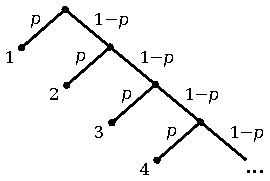
\includegraphics[width=0.4\textwidth]{img/Pfadbaum-zur-Anzahl.pdf}
\end{center}
\caption{Pfadbaum zur Anzahl}
\label{fig:Pfadbaum-zur-Anzahl}
\end{figure}

\vfill\noindent
\texttt{Dieses Heft steht unter der Creative-Commons-Lizenz CC0.}

\end{document}


